\documentclass[border=3pt]{standalone}
% Preâmbulo compartilhado pelos diagramas TikZ da aula 13 (SLAM com EKF)
\usepackage[T1]{fontenc}
\usepackage[utf8]{inputenc}
\usepackage{lmodern}
\usepackage{amsmath}
\usepackage{xcolor}
\usepackage{tikz}
\usetikzlibrary{arrows.meta,angles,quotes,decorations.pathmorphing,decorations.pathreplacing,calc,
                positioning,shapes.geometric,shapes.misc,backgrounds,fit,
                math}

% Paleta (mesma dos SVGs originais)
\definecolor{dblue}{HTML}{2A5B8C}
\definecolor{dorange}{HTML}{B3541E}
\definecolor{dgreen}{HTML}{4A7C59}
\definecolor{dred}{HTML}{9C4B4B}
\definecolor{dcream}{HTML}{F4F1EA}
\definecolor{dshade}{HTML}{DDD7C9}

% Função gaussiana (não normalizada por padrão de escala visual)
\pgfmathdeclarefunction{gauss}{3}{%
  \pgfmathparse{1/(#3*sqrt(2*pi))*exp(-((#1-#2)^2)/(2*#3^2))}%
}

% Estilos comuns (prefixo d... para não colidir com chaves internas do pgf)
\tikzset{
  >={Stealth[length=2mm]},
  dguide/.style={gray!55, dashed, line width=0.4pt},
  daxis/.style={gray!60, line width=0.7pt, ->},
  dbody/.style={fill=black!3, draw=black!80, line width=1pt},
  dacc/.style={draw=dblue, line width=1pt},
  dlbl/.style={black!55, font=\small},
  dsub/.style={black!45, font=\footnotesize},
  dstate/.style={circle, draw=black!80, fill=dcream, line width=1pt,
                 minimum size=17mm, font=\large, inner sep=1pt},
  dobs/.style={circle, draw=black!80, fill=dshade, line width=1pt,
               minimum size=14mm, font=\large, inner sep=1pt},
  dbox/.style={rounded corners=2pt, draw=black!80, fill=dcream, line width=1pt,
               align=center, inner sep=6pt},
  dop/.style={circle, draw=black!80, fill=white, line width=1pt,
              minimum size=6mm, inner sep=0pt, font=\small},
  dtrans/.style={->, dblue, line width=1pt},
  dmeas/.style={->, dorange, line width=1pt},
  dcurve/.style={line width=1pt, dblue},
  dcurveb/.style={line width=1.4pt, dorange},
}

\begin{document}
\hyphenpenalty=10000 \exhyphenpenalty=10000 \tolerance=9999 \emergencystretch=3em
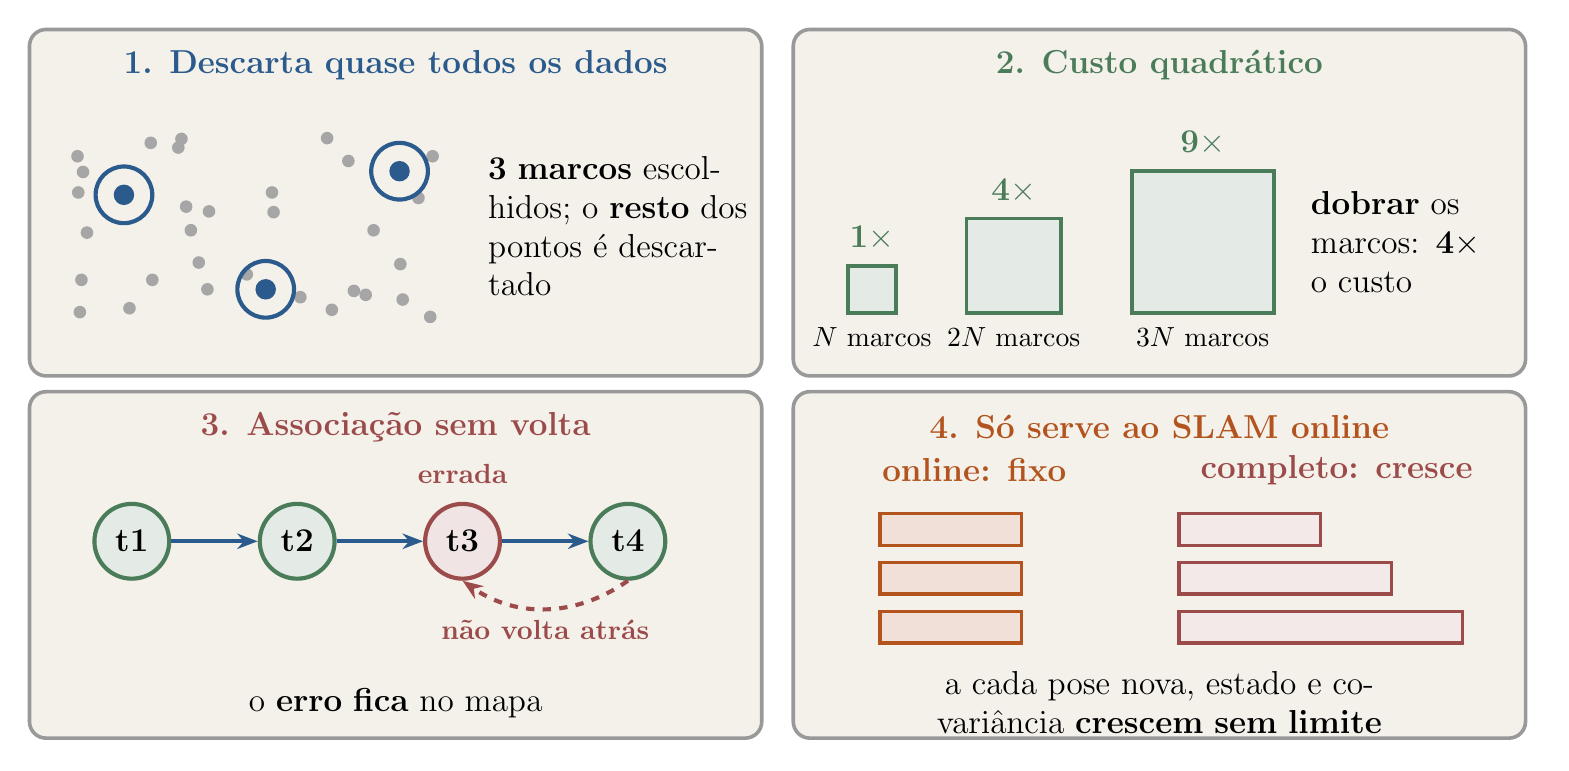
\begin{tikzpicture}[x=1cm,y=1cm]
\draw[black!40, line width=1.3pt, rounded corners=6pt, fill=dcream] (0.0,4.6) rectangle (9.3,9.0);
\node[font=\large\bfseries, text=dblue] at (4.65,8.55) {1. Descarta quase todos os dados};
\draw[black!40, line width=1.3pt, rounded corners=6pt, fill=dcream] (9.7,4.6) rectangle (19.0,9.0);
\node[font=\large\bfseries, text=dgreen] at (14.35,8.55) {2. Custo quadrático};
\draw[black!40, line width=1.3pt, rounded corners=6pt, fill=dcream] (0.0,0.0) rectangle (9.3,4.4);
\node[font=\large\bfseries, text=dred] at (4.65,3.95) {3. Associação sem volta};
\draw[black!40, line width=1.3pt, rounded corners=6pt, fill=dcream] (9.7,0.0) rectangle (19.0,4.4);
\node[font=\large\bfseries, text=dorange] at (14.35,3.95) {4. Só serve ao SLAM online};
\fill[black!35] (0.73,6.42) circle (0.08);
\fill[black!35] (4.94,6.86) circle (0.08);
\fill[black!35] (4.74,5.57) circle (0.08);
\fill[black!35] (2.76,5.89) circle (0.08);
\fill[black!35] (3.1,6.68) circle (0.08);
\fill[black!35] (0.66,5.82) circle (0.08);
\fill[black!35] (1.89,7.5) circle (0.08);
\fill[black!35] (4.12,5.68) circle (0.08);
\fill[black!35] (4.27,5.63) circle (0.08);
\fill[black!35] (3.44,5.6) circle (0.08);
\fill[black!35] (0.61,7.39) circle (0.08);
\fill[black!35] (1.56,5.82) circle (0.08);
\fill[black!35] (5.12,7.39) circle (0.08);
\fill[black!35] (1.93,7.61) circle (0.08);
\fill[black!35] (3.08,6.93) circle (0.08);
\fill[black!35] (1.54,7.56) circle (0.08);
\fill[black!35] (3.78,7.62) circle (0.08);
\fill[black!35] (4.71,6.02) circle (0.08);
\fill[black!35] (2.26,5.7) circle (0.08);
\fill[black!35] (1.27,5.46) circle (0.08);
\fill[black!35] (1.99,6.75) circle (0.08);
\fill[black!35] (0.62,6.93) circle (0.08);
\fill[black!35] (2.15,6.04) circle (0.08);
\fill[black!35] (4.37,6.45) circle (0.08);
\fill[black!35] (2.05,6.45) circle (0.08);
\fill[black!35] (3.84,5.44) circle (0.08);
\fill[black!35] (5.09,5.35) circle (0.08);
\fill[black!35] (4.05,7.33) circle (0.08);
\fill[black!35] (0.68,7.19) circle (0.08);
\fill[black!35] (2.28,6.69) circle (0.08);
\fill[black!35] (0.64,5.41) circle (0.08);
\fill[dblue] (1.2,6.9) circle (0.13); \draw[dblue, line width=1.5pt] (1.2,6.9) circle (0.36);
\fill[dblue] (3.0,5.7) circle (0.13); \draw[dblue, line width=1.5pt] (3.0,5.7) circle (0.36);
\fill[dblue] (4.7,7.2) circle (0.13); \draw[dblue, line width=1.5pt] (4.7,7.2) circle (0.36);
\node[font=\large, text width=3.3cm, align=left, anchor=west] at (5.7,6.5) {\textbf{3 marcos} escolhidos; o \textbf{resto} dos pontos é descartado};
\draw[dgreen, fill=dgreen!15, line width=1.4pt] (10.4,5.4) rectangle (11.0,6.0);
\node[font=\large\bfseries, dgreen] at (10.7,6.35) {1$\times$};
\node[font=\normalsize] at (10.7,5.1) {$N$ marcos};
\draw[dgreen, fill=dgreen!15, line width=1.4pt] (11.9,5.4) rectangle (13.1,6.6);
\node[font=\large\bfseries, dgreen] at (12.5,6.95) {4$\times$};
\node[font=\normalsize] at (12.5,5.1) {$2N$ marcos};
\draw[dgreen, fill=dgreen!15, line width=1.4pt] (14.0,5.4) rectangle (15.8,7.2);
\node[font=\large\bfseries, dgreen] at (14.9,7.55) {9$\times$};
\node[font=\normalsize] at (14.9,5.1) {$3N$ marcos};
\node[font=\large, text width=2.8cm, align=left, anchor=west] at (16.15,6.3) {\textbf{dobrar} os marcos: \textbf{4$\times$} o custo};
\node[circle, draw=dgreen, fill=dgreen!15, line width=1.5pt, minimum size=0.95cm, font=\large\bfseries] (q0) at (1.3,2.5) {t1};
\node[circle, draw=dgreen, fill=dgreen!15, line width=1.5pt, minimum size=0.95cm, font=\large\bfseries] (q1) at (3.4000000000000004,2.5) {t2};
\node[circle, draw=dred, fill=dred!15, line width=1.5pt, minimum size=0.95cm, font=\large\bfseries] (q2) at (5.5,2.5) {t3};
\node[circle, draw=dgreen, fill=dgreen!15, line width=1.5pt, minimum size=0.95cm, font=\large\bfseries] (q3) at (7.6000000000000005,2.5) {t4};
\draw[dtrans, line width=1.6pt, -{Stealth[length=2.6mm]}] (q0.east) -- (q1.west);
\draw[dtrans, line width=1.6pt, -{Stealth[length=2.6mm]}] (q1.east) -- (q2.west);
\draw[dtrans, line width=1.6pt, -{Stealth[length=2.6mm]}] (q2.east) -- (q3.west);
\node[font=\normalsize\bfseries, dred] at (5.5,3.35) {errada};
\draw[dred, dashed, line width=1.5pt, -{Stealth[length=2.6mm]}] (q3.south) to[bend left=35] node[below, font=\normalsize\bfseries, dred] {não volta atrás} (q2.south);
\node[font=\large, text width=7.6cm, align=center] at (4.65,0.45) {o \textbf{erro fica} no mapa};
\node[font=\large\bfseries, dorange] at (12.0,3.4) {online: fixo};
\node[font=\large\bfseries, dred] at (16.6,3.4) {completo: cresce};
\draw[dorange, fill=dorange!18, line width=1.2pt] (10.8,2.45) rectangle (12.6,2.85);
\draw[dred, fill=dred!12, line width=1.2pt] (14.6,2.45) rectangle (16.4,2.85);
\draw[dorange, fill=dorange!18, line width=1.2pt] (10.8,1.83) rectangle (12.6,2.23);
\draw[dred, fill=dred!12, line width=1.2pt] (14.6,1.83) rectangle (17.3,2.23);
\draw[dorange, fill=dorange!18, line width=1.2pt] (10.8,1.21) rectangle (12.6,1.61);
\draw[dred, fill=dred!12, line width=1.2pt] (14.6,1.21) rectangle (18.2,1.61);
\node[font=\large, text width=8.4cm, align=center] at (14.35,0.45) {a cada pose nova, estado e covariância \textbf{crescem sem limite}};
\end{tikzpicture}
\end{document}
